\documentclass[11pt]{article}
\usepackage{url}
\usepackage{cite}
\usepackage{amsmath}
\usepackage{graphicx}
\graphicspath{{../../umlet/}}

\begin{document}

\title{Top Down Parsing}
\author{Ernest Kirstein}
\maketitle

Historically, recursive descent parsers have been coded manually or else generated from 
a context free grammar specification. \cite{lewis, formal_langs} 
Coding a RDP manually is tedious, error prone, and difficult to maintain.
Programatically generating a RDP from a grammar
still isn't ideal - converting a context free grammar into
a recursive decent parsable form may not preserve the {\em strong equivalence} of the grammar.
And as a result, parse trees generated by that RDP will not be in the same form
as they might appear in the initial (non-RD-parsable) grammar, which is often a more 
natural representation of the desired language \cite{compiler}.

In this paper, I hope to describe a useful variation on recursive descent parseing
which addresses these problems. My system compiles a context free grammar 
specification into a RD-parseable grammar.
A parser is generated from the RD-parseable gramar,
and used to parse a input streams. 
The resulting parse trees are then transformed back into equivalent
parse trees under the original grammar. (Figure \ref{fig:high_level})

\begin{figure}[h!]
    \centering
    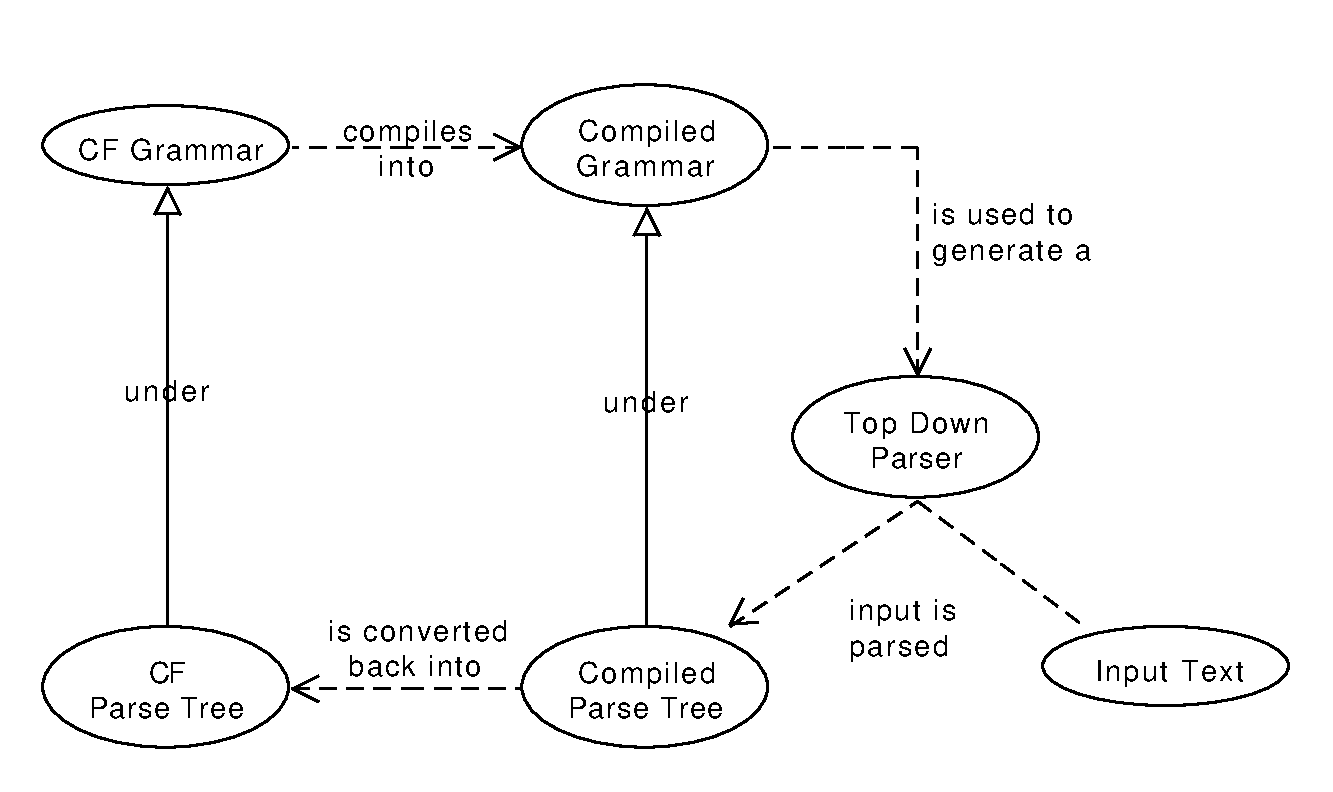
\includegraphics[width=0.9\textwidth,natwidth=1,natheight=1]{high_level.pdf}
    \caption{A high level overview of the process.}
    \label{fig:high_level}
\end{figure}

\clearpage

\section{Recursive Descent without Syntax Diagrams}
\label{rd_wo_sd}
Introductory material by Dr. Lewis \cite{lewis} describes a RDP as a piece of software which takes 
a sentence and turns it into a parse tree by performing a 'depth-first' search. 
But a search of what? One might try to call it a search of the parse tree, but that's not exactly right.
The 'recursive descent' name comes from the way that a RDP traverses through a
syntax diagram of a context free grammar \cite{compiler}.
The recursive descent algorithm in this paper does not use sytax diagrams (in hindsight,
this was a questionable design choice). This section will describe
how recursive descent parsing works without using syntax diagrams.

Consider a context-free grammar with the following production rules:
\setcounter{equation}{0}
\begin{align}
S &\rightarrow a S\\
S &\rightarrow b S\\
S &\rightarrow \epsilon
\end{align}
And the following string which we will attempt to parse: "ab"

We know, right off the bat, that the start symbol $S$ will be the root of any parse tree created under this
grammar, by virtue of it being the start symbol. (Figure \ref{fig:rdp_0})

\begin{figure}[h!]
    \centering
    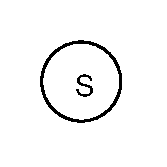
\includegraphics[natwidth=15,natheight=15]{rdp_0.pdf}
    \caption{Parse Tree 0}
    \label{fig:rdp_0}
\end{figure}

The next parse tree we should consider is the parse tree that is generated when we follow the first 
production rule. (Figure \ref{fig:rdp_1}) Notice that, in this instance, the parse tree does not conflict with
the string we are trying to parse - i.e. regardless of the production rules we follow the string that is
produced from any further production rules we follow will start with "a".

\begin{figure}[h!]
    \centering
    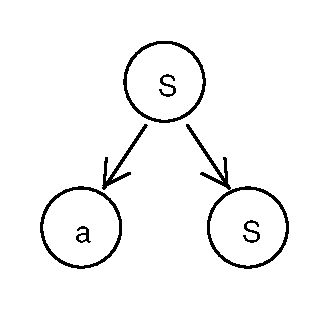
\includegraphics[width=0.4\textwidth,natwidth=30,natheight=30]{rdp_1.pdf}
    \caption{Parse Tree 1 - Valid}
    \label{fig:rdp_1}
\end{figure}

For the next parse tree, we will try to repeat are last action (following the first possible production rule).
(Figure \ref{fig:rdp_2}) This parse tree conflicts with the string we are trying to produce since any
string produced by further production rule applications will produce a string starting with "aa".
In this case, we go back to the previous parse tree and try a different production rule.

\begin{figure}[h!]
    \centering
    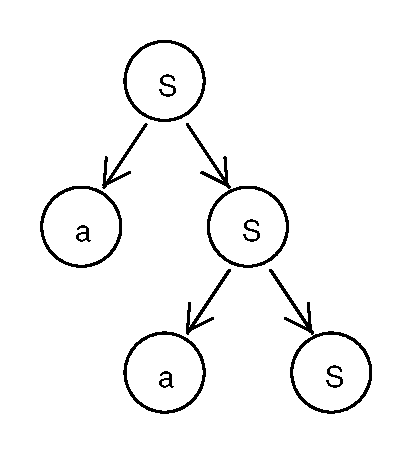
\includegraphics[width=0.4\textwidth,natwidth=30,natheight=30]{rdp_2.pdf}
    \caption{Parse Tree 2 - Invalid}
    \label{fig:rdp_2}
\end{figure}

In figure \ref{fig:rdp_3}, we've followed the second production rule
and our new parse tree fits with the input string, so we can continue our descent.

\begin{figure}[h!]
    \centering
    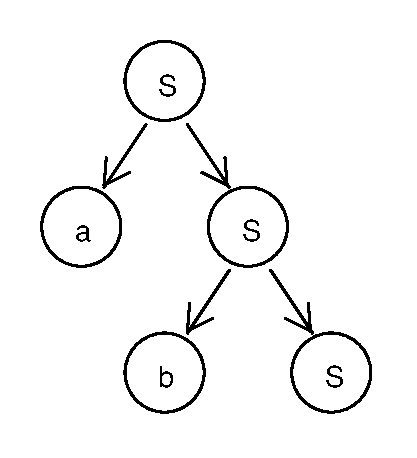
\includegraphics[width=0.4\textwidth,natwidth=30,natheight=30]{rdp_3.pdf}
    \caption{Parse Tree 3 - Valid}
    \label{fig:rdp_3}
\end{figure}

The next two parse trees (Figure \ref{fig:rdp_4_5}), created by applying the first and second production rules to
Parse Tree 3, are both invalid because they extend past the length of our input string.

\begin{figure}[h!]
    \centering
    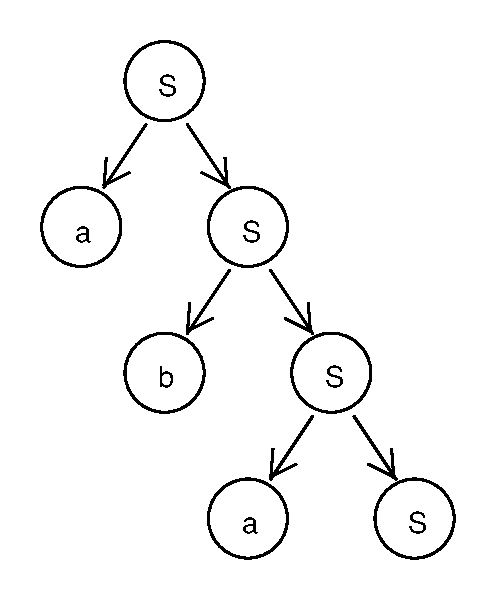
\includegraphics[width=0.4\textwidth,natwidth=30,natheight=30]{rdp_4.pdf}
    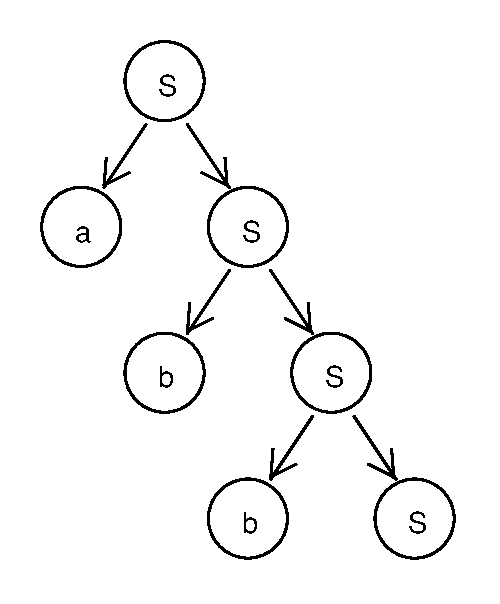
\includegraphics[width=0.4\textwidth,natwidth=30,natheight=30]{rdp_5.pdf}
    \caption{Parse Trees 4 and 5 - Both Invalid}
    \label{fig:rdp_4_5}
\end{figure}

In the last step, by applying the third production rule to Parse Tree 3, we have a parse tree which terminates and produces the
desired input string, "ab". (Figure \ref{fig:rdp_6})

\begin{figure}[h!]
    \centering
    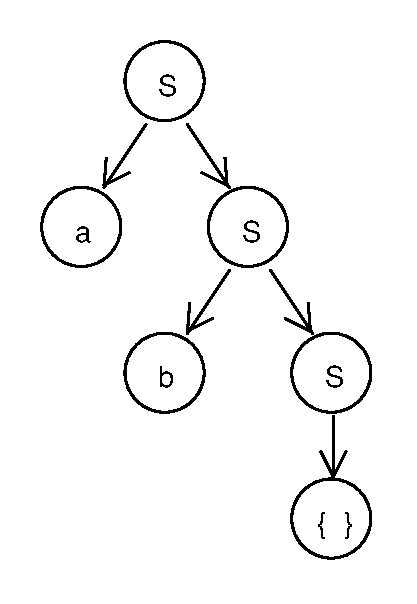
\includegraphics[width=0.4\textwidth,natwidth=30,natheight=30]{rdp_6.pdf}
    \caption{Parse Tree 6 - Complete}
    \label{fig:rdp_6}
\end{figure}

Finally, let's diagram our traversal through the possible parse trees (Figure \ref{fig:rdp_7}). Shown this way, one can notice
a pattern in our attempt to build the tree. The recursive descent parser performs a depth first search of the 
graph of possible parse trees, looking for a parse tree which fits the input string.
The child nodes from each PT (Parse Tree) node in the graph are PT nodes generated by
applying each of the production rules to the first (left, deepest) nonterminal symbol in that PT node.
The depth of each node in the PT tree corresponds with the number of production rules that have been applied.

\begin{figure}[h!]
    \centering
    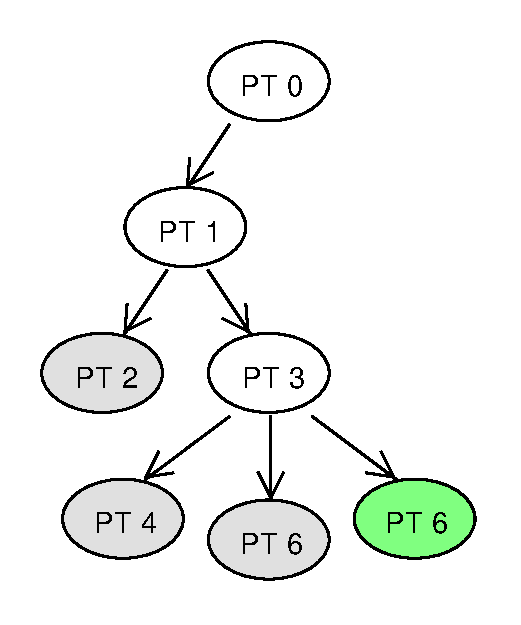
\includegraphics[width=0.4\textwidth,natwidth=30,natheight=30]{rdp_7.pdf}
    \caption{Parse Tree Search Progression}
    \label{fig:rdp_7}
\end{figure}

\clearpage

\section{Effect of Grammar Transformations on Parse Trees}
Left recursion is a problem for recursive descent parsers because it causes them to
go into an infinite loop. Using the model described in section \ref{rd_wo_sd}:
when a PT node is reach where the first non-terminal symbol has a production rule with
left recursion, it's child node will have the same non-terminal symbol so it will produce
a child node with the same non-terinal symbol ad infinitum - and none of those children will
consume any terminals from the input stream so the parser will not proceed. 

So, removing left recursion from context free grammars is a necessary evil for recursive descent parsing.
It just takes two transformations to turn any context free grammar with left recursion
into a {\em weakly equivalent} grammar with only right recursion.
These two transformations are direct left recursion elimination, 
$DLRE(G; R_\alpha, R_\beta) \rightarrow G'$ and substitution, 
$Sub(G; r_\alpha, R_\beta) \rightarrow G'$, which is used to
remove indirect left recursion. \cite{aho, lewis}
These sections will describe how these transformations work on the grammar
and on their parse trees.

\subsection{Direct Left Recursion Elimination}
A left recursive grammar, $G$, has rules for some non-terminal $A$ of the form
$A \rightarrow A \alpha_i$ and $A \rightarrow \beta_j$, $i \in [1,m]$, $j \in [1,n]$.
Let $R_\alpha$ and $R_\beta$ represent the sets of those rules respectively where the notation
$R_\alpha(1)$ represents $A \rightarrow A \alpha_1$. 
Such a grammar represents a language which contains strings of the form
$\beta_y \alpha_{x_1} \alpha_{x_2} ... \alpha_{x_p}...\alpha_{x_{k-1}} \alpha_{x_k}$ where $y \in [1,m]$ and each $x_p \in [1,n]$.
However, to produce such a string, the alpha rules need to be followed in reverse order:
\[R_\alpha(x_k), R_\alpha(x_{k-1}), ... R_\alpha(x_{p}), ... R_\alpha(x_2), R_\alpha(x_1), R_\beta(y)\]

The transformation \cite{aho} $DLRE(G; R_\alpha, R_\beta) \rightarrow G'$ changes
each rule in $R_\alpha$ to the form $A' \rightarrow \alpha_i A'$, each rule
in $R_\beta$ to the form $A \rightarrow \beta_j A'$, and adds an additional rule
$R_\epsilon = A' \rightarrow \epsilon$. Consequently, the order of the followed production
rules in $G'$ results in alpha rules being followed in forward order:

\[R_\beta(y), R_\alpha(x_1), R_\alpha(x_2), ... R_\alpha(x_p), ... R_\alpha(x_{k-1}),R_\alpha(x_k), R_\epsilon \]


\begin{figure}[h!]
    \centering
    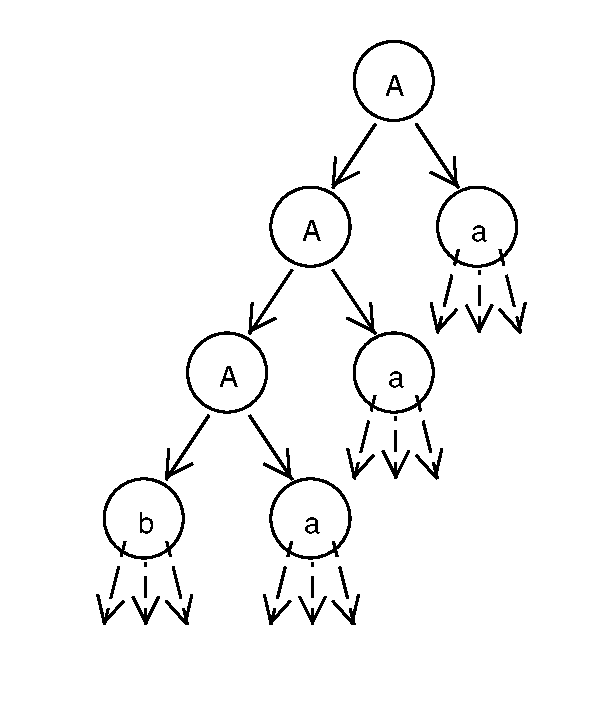
\includegraphics[width=0.4\textwidth,natwidth=1,natheight=1]{dlre_orig.pdf}
    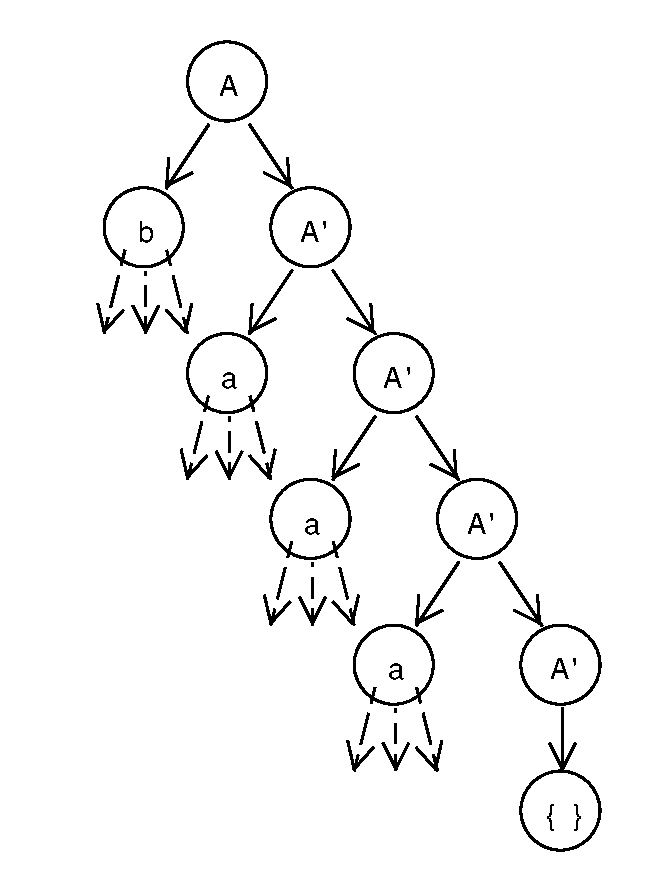
\includegraphics[width=0.4\textwidth,natwidth=1,natheight=1]{dlre_comp.pdf}
    \caption{Original and Transformed Parse Trees}
    \label{fig:dlre}
\end{figure}

The transformation effects the parse trees by flipping and reversing $A$ chains,
replacing lower $A$ nodes with $A'$ nodes, moving the $\beta$ up,
and adding an $A'$ node and $\epsilon$ node to the end of the chain. (Figure \ref{fig:dlre}) The inverse transformation
removes last $A'$ and $\epsilon$ nodes, moves the $\beta$ back down to the end of the chain, and changes the $A'$ nodes back into
$A$ nodes, then flips and reverses the $A$ chain. Note that the $\alpha$ and $\beta$ nodes are arbitrary strings, so in reality
they might be multiple nodes which might have any number of children.

More formally, for each $A$ node in the RD-parsable grammar, the inverse transformation $DLRE^{-1}(T'; A, A') \rightarrow T$
modifies chains of $A/A'$ nodes where the children of the $A$ node are $C_A$, of all but the last $A'_{x_p}$ node are $C_{A'_{x p}}$,
and the last $A'_\epsilon$ node has only the child $\epsilon$.
From the $DLRE$ transformation rules we know that the $C_A$ will be of the form $\beta_y A'_{x_1}$. 
We can also conclude from the $DLRE$ tranformation that each $C_{A'_{x p}}$ will be of the form $\alpha_p A'_{x_{p+1}}$
when $p < k$ and $A'_\epsilon$ when $p=k$. 

The inverse transformation first removes the $A'_\epsilon$ node. Then it changes each remaining $A'_{x_p}$ node into an $A_{x_p}$ node
with the same children. Next the $A_{x_p}$ are restructured such that each $C_{A_{x p}}$
is equal to $A_{x_{p-1}} \alpha_p$ where $1 < p$ and $\beta_y \alpha_k$ where $p=1$. The top node of the chain, 
$A$, is replaced with $A_{x_k}$. And this process is repeated for each chain.

\subsection{Substitution}

TODO

\clearpage

\section{Compiling a Context Free Grammar for RD Parsing}

It is important to notice that not all context free grammars can be directly parsed by
recursive descent. Some context free grammars require a bit of maniuplation to remove
left recursion (direct or otherwise) \cite{compiler}. This process of converting a context
free grammar into a {\em weakly equivalent} recursive descent parsable grammar shall be refered to as
{\em compiling} the grammar.

In this section, a grammar will be define from an ordered collection of production rules.
My parser uses context-free grammar rules, which are comprised of a
'head' (the single-symbol left hand side of the production rule), and a 'tail'
(one or more symbols comprising the right hand side of the production rule).

These grammars may be 'compiled' using the four procedures:
factoring, substitution, removing left recursion, and removing useless
rules. Let 'decision list' define an ordered list of production rule
choices which produces a parse tree.
As each of these four procedures produces a weakly equivalent grammar,
there exists a mapping for any decision list in a compiled grammar
back into a same-terminal-producing decision list in the pre-compiled (parent) grammar.
My parser keeps track of these inverse transformation rules as performs
it's compilation procedure so that a compiled grammar's decision list can be easily
converted to the initial grammar's equavalent decision list. 

Take this simple grammar for example:
\setcounter{equation}{0}
\begin{align}
S &\rightarrow A B\\
A &\rightarrow a\\
A &\rightarrow S A\\
B &\rightarrow b\\
B &\rightarrow S B
\end{align}
It compiles into the weakly equivalent grammar:
\setcounter{equation}{0}
\begin{align}
Z &\rightarrow \epsilon\\
B &\rightarrow b\\
S &\rightarrow a B S'\\
S' &\rightarrow \epsilon\\
A &\rightarrow a Z\\
B &\rightarrow a B S' B\\
S' &\rightarrow a Z B S'\\
Z &\rightarrow b S' A\\
Z &\rightarrow a B S' B S' A
\end{align}

So when the terminal stream "aabb" is parsed in the compiled
grammar to the decision list $[3, 6, 2, 4, 2, 4]$ it can be transformed
into the parent-grammar-equivalent decision list: $[1, 2, 5, 1, 2, 4, 4]$.

\begin{figure}[h!]
    \centering
    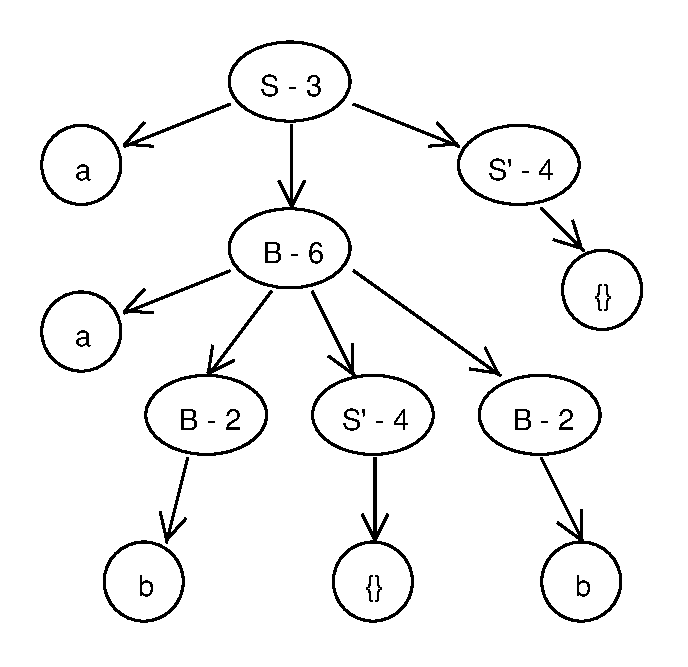
\includegraphics[width=0.4\textwidth,natwidth=458,natheight=444]{compiled_ex.pdf}
    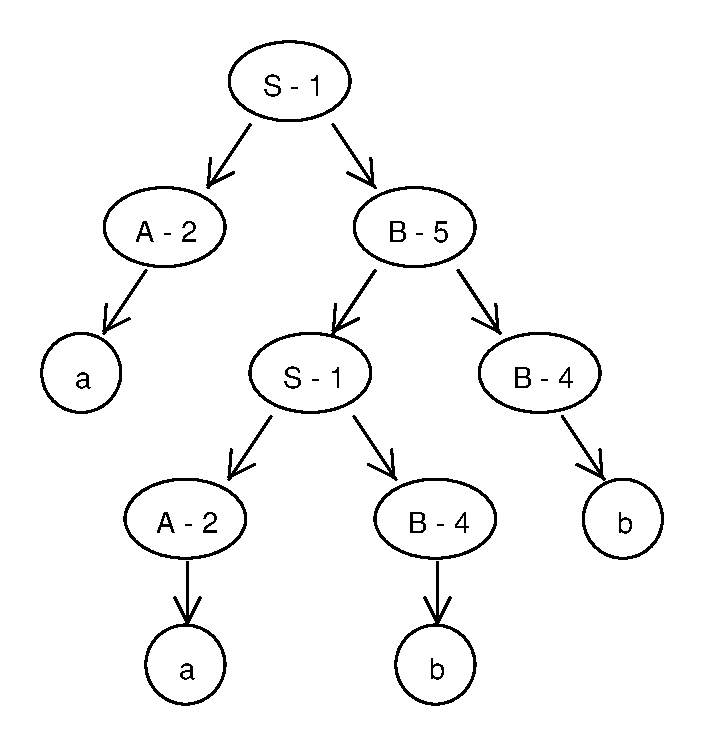
\includegraphics[width=0.4\textwidth,natwidth=472,natheight=500]{decompiled_ex.pdf}
    \caption{Compiled Grammar Parse Tree (left) Parent Grammar Parse Tree (right)}
    \label{fig:comp_to_dec_ex}
\end{figure}

\clearpage

\section*{Terms}

\begin{itemize}
\item \textbf{Grammar}: a phrase-structure grammar is defined by a finite vocabulary (alphabet), a finite set of
initial strings, and a finite set of rules... \cite{chomsky} (see Production Rule)
\item \textbf{Context-Free Grammar}: a context free grammar is one which only has production rules whose head is a single non-terminal symbol.
\cite{compiler, anatomy, formal_langs}
\item \textbf{Production, Production Rule, Rewrite Rule}: rules of the form $X \rightarrow Y$ where
$X$ and $Y$ are strings in [a grammar]  \cite{chomsky};
define the nonterminal symbols by sequences of terminals and nonterminal symbols \cite{compiler};
rules which specify how nonterminal symbols may be expanded into new sequences of symbols (terminal or otherwise).
\item \textbf{Head (Production Rule)}: the left hand side of a production rule
\item \textbf{Tail (Production Rule)}: the right hand side of a production rule
\item \textbf{Parse Tree}: an ordered, rooted tree whose nodes are symbols in a context-free grammar where the 
children of each brach node correspond to the tail of some production rule in said grammar;
a tree-representation of the grammatical structure of [an input stream] \cite{anatomy}
\item \textbf{Weakly Equivalent (Grammar)}: two grammars are [weakly] equivalent if they define the same language.\cite{reghizzi}
\item \textbf{Strongly/Structurally Equivalent (Grammar)}: two grammars are strongly or structurally equivalent
if they are weakly equivalent and can assign any sentence the same parse tree. \cite{reghizzi}
\end{itemize}


\bibliography{notes}{}
\bibliographystyle{plain}
\end{document}
